\documentclass[a4paper,12pt]{article}

\usepackage[left=2.5cm, right=2.5cm, top=3cm, bottom=3cm]{geometry}
\usepackage{amsmath, amsthm, amssymb}
\usepackage[spanish]{babel}
\usepackage{cite}
\usepackage{graphicx}
\usepackage{url}

\bibliographystyle{plain} 

\begin{document}
\title{Presentacion}
\author{Glenda Natalí Ríos Rodríguez}
\date{Julio, 2023}
\maketitle

\begin{abstract}
   A continuación y de forma muy breve tratare de explicar la utilidad de mi propuesta de MOOGLE!
   y dare una pequeña guia para el usuario que quiera emplearla.  
\end{abstract}

\section{¿Que es MOOGLE! ?}\label{sec:intro}

MOOGLE! es un programa que pretende sobre una base de datos de tipo .txt realizar
una busqueda inteligente segun una frase o expresion que introduce el usuario a la cual
llamaremos Query.
El usuario obtendra como respuesta una lista con los documentos contenidos en la base de
datos que estan relacionados con la query ; dicha lista estara ordenada de mayor a menor
segun la relevancia que tengan los documentos con la query. Ademas se mostrata un pequeño
fragmento del documento en la que se le hace referencia a la query.


\section{Guia para el usuario}\label{sec:ent}


\subsection{Pasos a seguir por el usuario para realizar una busqueda en MOOGLE! :
}

\begin{enumerate}
    \item Escribir la query en la barra de busqueda. 
    \item Presione el boton de busqueda.
    \begin{enumerate}
        \item Si su consulta es vacía aparecerá en pantalla el texto
        “No existen Documentos relacionados con su Consulta”.
        \item Si al realizar la busqueda no se encuentra ningun documento que guarde 
        relacion con la Query entonces aparecerá en pantalla“No existen Documentos relacionados
        con su Consulta”.
    \end{enumerate}
\end{enumerate}

\subsection{Como personalizar la busqueda:}

\begin{itemize}
    \item En la query , al ponerle \textbf{!} delante a una palabra \textbf{(sin separarlo por un espacio)} el programa realizara la busqueda normal pero solo mostrara los documentosque no contienen dicha palabra.   
    \item En la query , al ponerle \textbf{\^{}} delante a una palabra \textbf{(sin separarlo por un espacio)} el programa realizara la busqueda normal pero solo mostrara los documentos que contienen dicha palabra. 
    \item En la query , al ponerle \textbf{*} delante a una palabra \textbf{(sin separarlo por un espacio)} el programa a la hora de realizar la busqueda le dara mas peso a dicha palabra \textbf{(mientras mas * le pongamos delante a la palabra mas peso tendra esta en la busqueda)}
    \item Se puede utilizar una combinacion de estos simbolos para hacer mas especificas las busquedas , pero esta claro que \textbf{no se puede poner ! y \^{} delante de una misma palabra}
\end{itemize}

\begin{figure}[h]
    \centering
    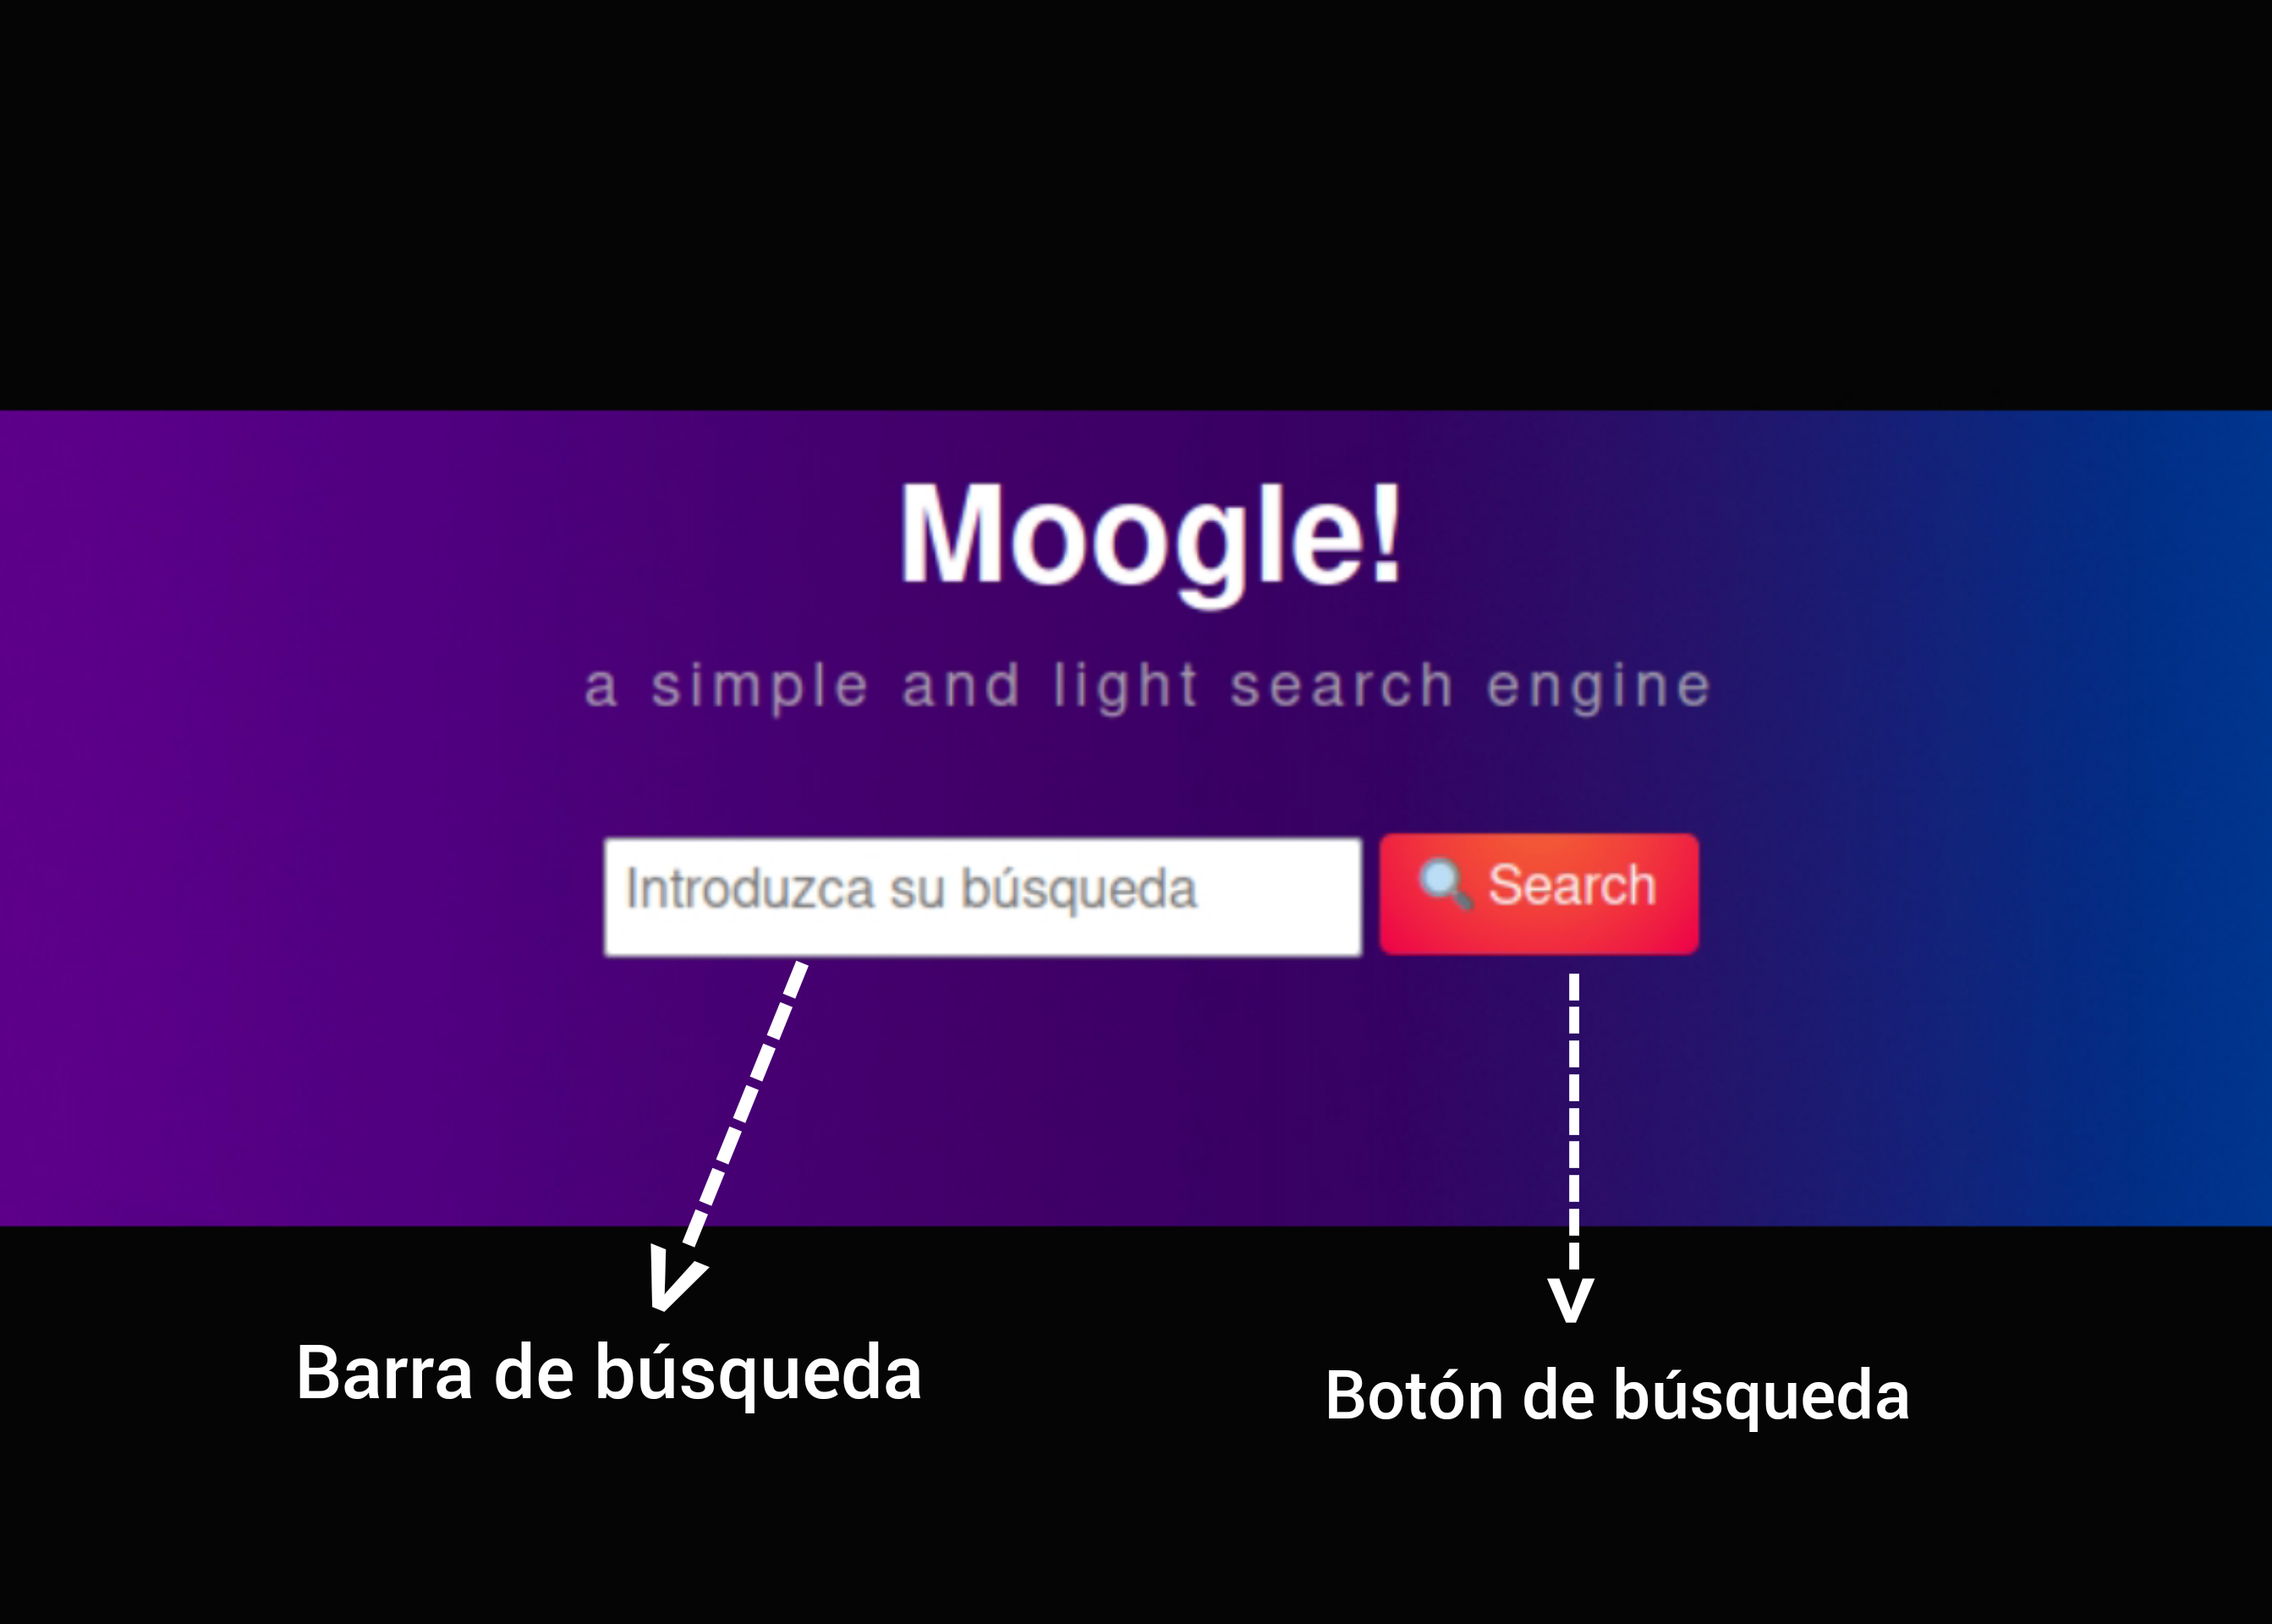
\includegraphics[width=\textwidth]{imagenes/ejemplo.jpg}
\end{figure}

\end{document}
